\documentclass{article}

% Language setting
% Replace `english' with e.g. `spanish' to change the document language
\usepackage[english]{babel}

% Set page size and margins
% Replace `letterpaper' with `a4paper' for UK/EU standard size
\usepackage[letterpaper,top=1cm,bottom=2cm,left=2cm,right=2cm,marginparwidth=1.75cm]{geometry}

% Useful packages
\usepackage{amsmath}
\usepackage{graphicx}
\usepackage[colorlinks=true, allcolors=blue]{hyperref}

\title{CS3080 Final Project}
\author{Rachel Koch}

\begin{document}
\maketitle

\section{Conclusion and Results}

In Star Trek: The Next Generation (TNG), Data is an android who dreams of becoming more human. This project aimed to determine whether Data's speech patterns actually become more human throughout the show by analyzing how many different words Data used per episode. Linear regression analysis was performed on the total word counts to see if the overall trend was increasing over time, and the results proved inconclusive. The number of words used per episode was analyzed, and so was the average number of words used per season. Both showed a very slight positive slope, but accuracy numbers (R-Squared) were below 1\% [across episodes: 0\% - across seasons: 0.17\%].

This result is somewhat unsurprising when the data is graphed and examined. Looking at Figure 1, it can be seen that the data on number of unique words used per episode does not appear linear (top plot). The data on average number of words used per season seems more linear, but also seems to hover around the same value, rather than steadily increasing (bottom plot). As such, the linear regression analysis proved entirely inaccurate [$R^2 < 1\%$].

Simple Linear Regression Analysis assumes the data meets a few conditions: Linearity, Homoscedasticity, and Independent Errors. This data seems to fall afoul of at least the linearity assumption, so in hindsight, linear regression was not the best analysis to perform for this task. As can be seen when the linear regression lines were graphed (Figure 2), they show almost no change in average number of words across all 7 seasons of TNG. In the end, this analysis did not provide any useful data to accomplish our ultimate goal of determining whether Data's speech patterns became more human over time.

\begin{figure}[hbt!]
    \centering
    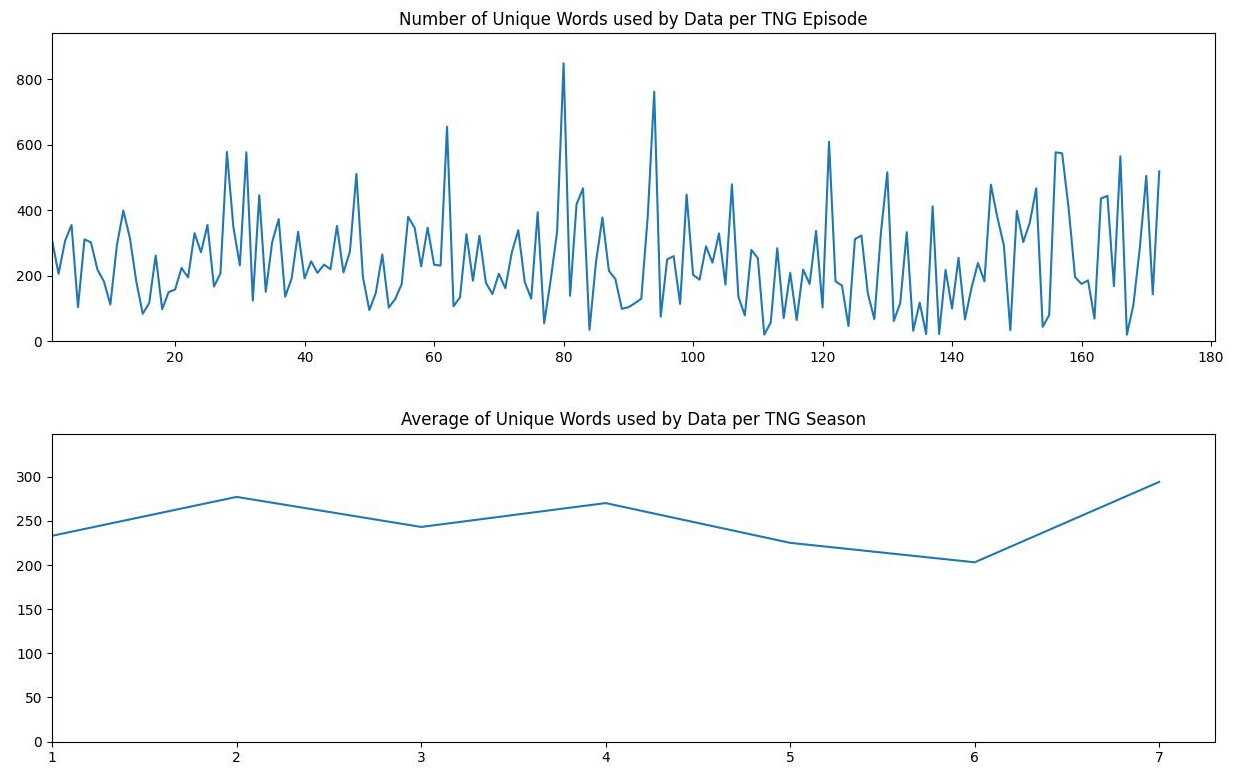
\includegraphics[width=0.75\linewidth]{Screenshot from 2024-07-27 12-03-41.png}
    \caption{Graphs of Initial Data}
    \label{fig:enter-label}
\end{figure}

The data for Data's speech required a good amount of cleaning up before the words were able to be accurately counted. Punctuation had to be removed, all upper case letters had to be converted to lower case so that, for example, 'The' and 'the' were counted as the same word. If these factors had not been accounted for, the results would have been different. Additionally, using a different form of analysis likely would have led to different results, as discussed in the next section.

\begin{figure}
    \centering
    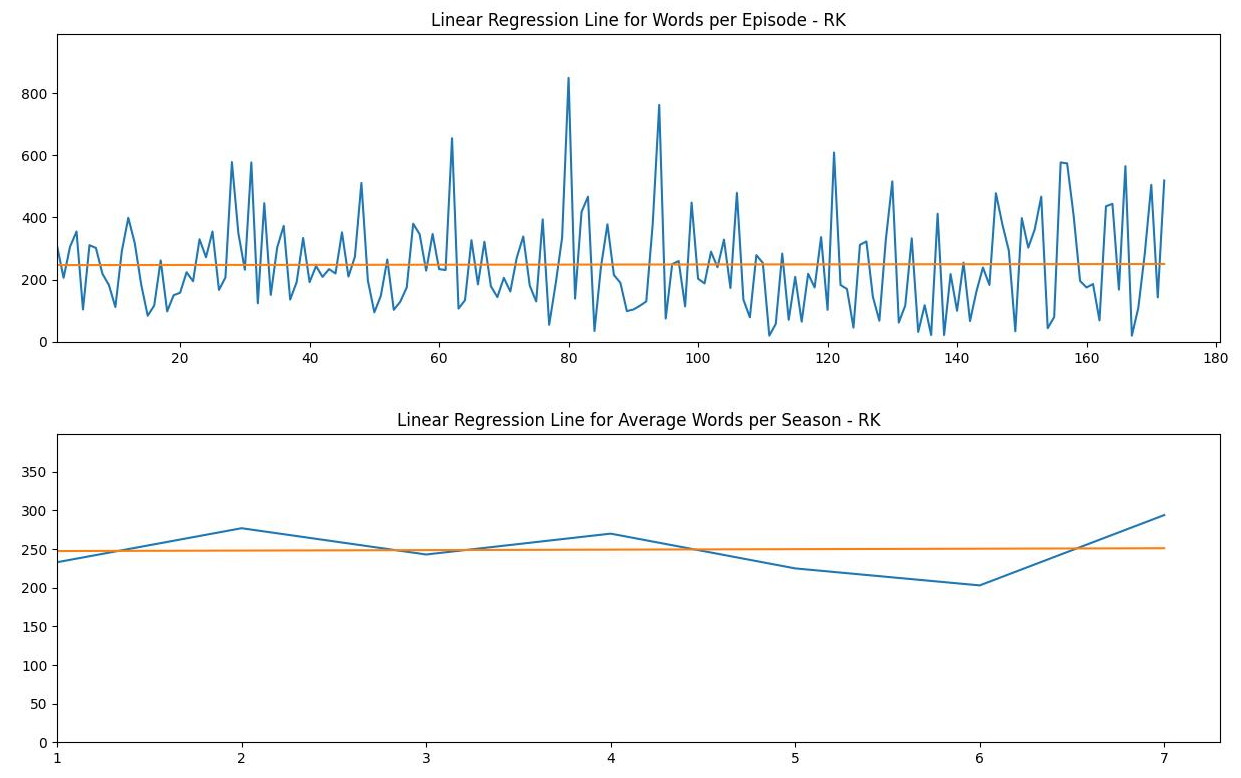
\includegraphics[width=0.75\linewidth]{Screenshot from 2024-07-27 12-53-24.png}
    \caption{Graphs Containing Linear Regression Lines}
    \label{fig:enter-label}
\end{figure}

\section{Possible Improvements and Future Testing}

The number of unique words spoken per episode appears to be periodic, which would lend itself better to a Fourier analysis. This might have revealed some patterns amongst the noise, which we struggle to see in the raw data. Even a weighted Regression analysis might have given us more information, by dividing each episode's word total by the total number of words spoken in the episode. This proves to be a more accurate measurement because it shows the ratio of unique words spoken per total number of words spoken. Preliminary results backed up this theory, but only minimally [$R^2$ results were still below 1\% (across episodes: 0.02\% - across seasons: 0.37\%)].

These tests also failed to take into consideration any industry or contextual factors. For example, the writers might have been required to make sure the actor spoke X number of times per episode/season. Also, actors are in different plot lines across episodes [the A plot (main plot line), the B plot (secondary plot line), or both]; which is something a Fourier analysis could help us better understand the affects of. And as a last consideration, that fact that humans wrote the script likely interfered with the hypothesis that we can use the same tools as are used when identifying AI vs. human writing.

\section{Manual Implementation of Linear Regression}

My manual implementation of Linear Regression provided the same results as the library functions did. I wrote functions that implemented the linear regression equations mathematically, and it seems like the Scikit-learn library works the same way. However, despite being more accessible, we generally do not know exactly how a library is working under the hood. As an example, I learned after several failed attempts of implementing this library that the x value array being passed into the Linear Regression function must be 2D - which is not obvious from the docs.

\section{Implications}

There are many ways to manipulate data presentation so that it looks the way we want it to. In section 2, I could have said that using weighted numbers increased my accuracy by 217\%! This would have been misleading though, because my overall accuracy was still under 1\%. We could also have sent in the data that only supports our desired outcome, filter out anything that doesn't contribute to our bottom line. The antidote for this is having the ability to run these algorithms yourself, then you don't have to just rely on what someone tells you. 

At the end of the day, if the source code is unavailable, only the people who programmed an AI model know how it works. Even then, if you have one person working on a part, and another person working on another part, then there may not be a single person who knows how it works. So it seems to be up to the reader to be critical when absorbing information, and only take in things that can be independently verified. Even better if you can test it yourself!

\end{document}